\documentclass[titlepage, a4paper, 12pt]{article}
\usepackage{graphicx}
\usepackage{caption}
\usepackage{hyperref}
\usepackage{fancyhdr}

\title{Use Case Specification\\ Project C}
\date{24-09-2018}

\author{0951234 - Ryan Graute\\ 0946132 - Tim Dallau\\ 0945599 - Casper de Keizer\\ 0956758 - Daniel Dudink}

\hypersetup{
    colorlinks,
    citecolor=black,
    filecolor=black,
    linkcolor=black,
    urlcolor=black
}

\begin{document}

\begin{titlepage}
	\maketitle
\end{titlepage}

\tableofcontents
\newpage

\section{Introduction}
\subsection{Purpose of this document}
This document servers as an overview for the use cases for Project C

\subsection{Scope}
The Scope of the project is to offer users a webshop to browse, search and order products. Users of the website can also register and sign up for an account on the webshop.
User that are signed in can view their order history and see the status of their orders. Having a registered account is required to place an order.\\
\newline
In the system there are also admin accounts. These admin accounts can create, edit and delete users and products.
\subsection{Project approach}
Scrum methodology will be used, because it allows for high flexibility in terms of adapting to the project owner’s demands and we believe the constant feedback loop will result in a better product.
\subsection{References}
\begin{itemize}
	\item Course manual. Can be found on lms.hr.nl
\end{itemize}
\subsection{Version control}

\begin{table}[ht]
	\centering
	\resizebox{\textwidth}{20pt}{\begin{tabular}{||c|c|c|c|c||}
		\hline
		Version & Status & Date & Author & Remarks\\
		\hline\hline
		0.1 & Concept & 21-09-2018 & Ryan Graute, Tim Dallau & \\
		\hline
		1.0 & Final & 24-09-2018 & Ryan Graute, Tim Dallau, Daniel Dudink Casper de Keizer & \\
		\hline
	\end{tabular}}
\end{table}

\subsection{Target audiance}
This document is for:
\begin{itemize}
	\item Product owner
	\item Developers
\end{itemize}

\newpage

\section{Summary actors}
\begin{table}[ht]
	\begin{tabular}{|c|c|}
		\hline
		Actor & Description\\
		\hline\hline
		Admin & System admin that has full control over the system.\\
		\hline
		Guest & User that can only browse products.\\
		\hline
		Registered User & User that can order products.\\
		\hline
		Payment System & System that takes care of the payment for the order.\\
		\hline
	\end{tabular}
\end{table}

\section{Summary use cases}
\begin{table}[ht]
	\centering
	\captionsetup{labelformat=empty}
	\begin{tabular}{|c|c|c|c|}
		\hline
		Use case name & Description & Importance & Priority\\
		\hline\hline
		Login & The User must be logged-in to order. & 3 & 3\\
		\hline
		Register & A guest must be able to create an account. & 3 & 3\\
		\hline
		Search Products & A user can search for products. & 3 & 2\\
		\hline
		Order Products & A user can order products & 3 & 3\\
		\hline
		View History & A logged in user van view his order history & 1 & 1\\
		\hline
		Add Product & An admin can add new products. & 3 & 3\\
		\hline
		Edit Product & An admin can edit products. & 2 & 2\\
		\hline
		Delete Product & An admin can delete products & 2 & 2\\
		\hline
		Add User & An admin can add a new user. & 3 & 3\\
		\hline
		Edit User & An admin can edit a user account. & 2 & 2\\
		\hline
		Delete User & An admin can delete a user account. & 2 & 2\\
		\hline
		View Statistics & The admin can view the statistics of the webshop. & 1 & 1\\
	\hline\end{tabular}
	\caption{The importance and priority have a value of 1 to 3, where 3 is the highest value (most important / highest priority).}
\end{table}

\newpage

\section{Use case diagram}
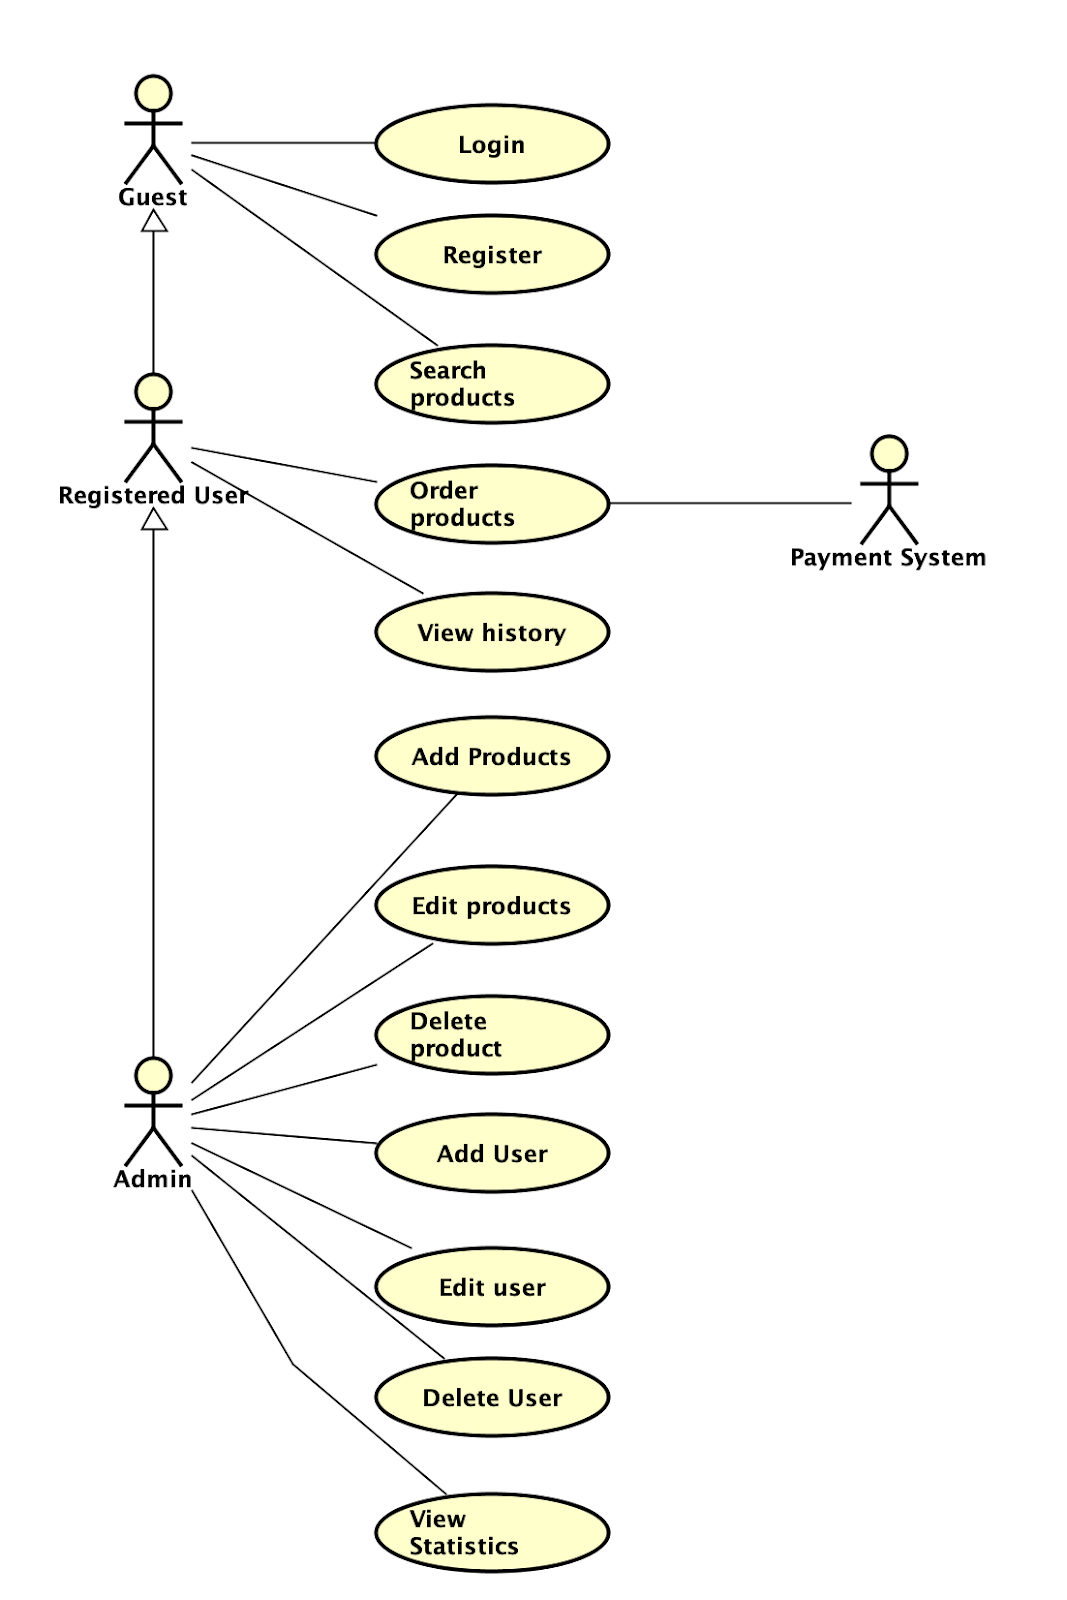
\includegraphics[width=0.80\linewidth]{images/use-case.png}

\section{Description use cases}
\subsection{Use case login}
\subsection{Use case Register}
\subsection{Use case search products}
\subsection{Use case order products}
\subsection{Use case view history}
\subsection{Use case add product}
\subsection{Use case add user}
\subsection{Use case edit product}
\subsection{Use case edit user}
\subsection{Use case delete product}
\subsection{Use case delete user}
\subsection{Use case view statistics}
\end{document}
